\section{Theorie}

Wird ein Festkörper mit Licht bestrahlt, werden unter gewissen Vorraussetzungen
Elektronen aus diesem gelöst. Dieses Phänomen wird im Versuch V500: "Der Photoeffekt"
untersucht.

Eine widerspruchsfreie Erklärung von Licht, erlaubt nur die Quantenelektrodynamik.
Dieses Modell beinhaltet den Wellencharakter und den Teilchencharakter von Licht
als Grenzfälle. Das Wellenmodell zur Beschreibung von Licht ist immer dann sinnvoll,
wenn über eine große Anzahl von Photonen gemittelt werden kann. Hingegen eigent
sich das Teilchenmodell zur Erklärung der Phänomene, wenn Licht mit Materie wechselwirkt.

Der Photoeffekt lässt sich mit Hilfe des Teilchcharakters anschaulich erklären.
Ein Photon trifft mit der Energie $\su{h}\nu$ auf ein in der Oberfläche befindliches
Elektron.
Überschreitet die Energie des Photons die Austrittsarbeit des Elektrons, wird
dieses aus der Oberfläche gelöst. Die Energiebillanz des Photoeffektes
sieht wie folgt aus:

\begin{equation}
  \label{eqn:Energiebillanz}
  \su{h}\nu = \su{E}\ua{kin} + \su{A}\ua{k}.
\end{equation}

Der Photoeffekt tritt unabhängig von der Intensität des Lichtes auf, nur die
Frequenz $\nu$ ist ausschlaggebend. Intensiveres Licht erhöht lediglich die
Anzahl der Photonen, sodass mehr Elektornen ausgelöst werden.

Der Photoeffekt kann mittels einer Photozelle (vgl. Abb. \ref{fig:Photozelle}) beobachtet werden.
Der Glaskolben der Photozelle ist evakuiert, sodass gelöste Elektronen nicht von
Luftmolekülen eingefangen werden können. Auf die Innenseite des Kolbens ist eine
Metallschicht aufgedampft, die die Kathode darstellt. Vor der Kathodenoberfläche
ist eine kreisförmige Anode angebracht, die auf gelöste Elektronen eine anziehende
Kraft ausübt.

\begin{figure}
  \centering
  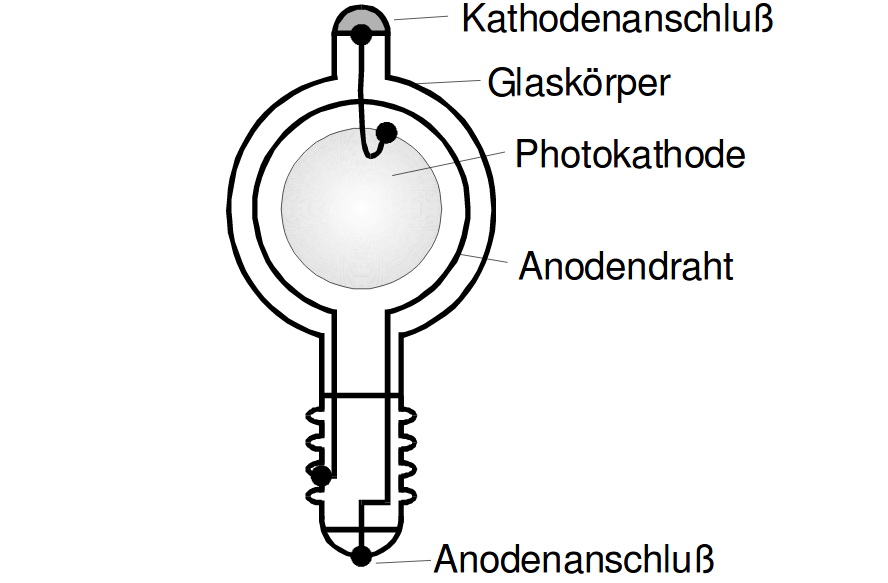
\includegraphics[width=9cm, height=7cm]{Pics/Photozelle.png}
  \caption{Schematische Darstellung einer Photozelle}
  \label{fig:Photozelle}
\end{figure}

Die gelösten Elektronen bilden einen Photostrom. Die Energie der Elektronen des Photostroms
kann durch die Gegenstrommethode bestimmt werden.
Dabei wird an den Kathodenanschluß und den Anodenanschluß (vgl. Abb. \ref{fig:Photozelle})
eine variable Spannung $\su{U}$ angelegt.
Wenn die angelegte Spannung den Photostrom kompensiert, gilt folgende Energierelation.

\begin{equation}
  \label{eqn:Gegenfeldmethode}
  e_0\su{U}\ua{g} = \frac{1}{2}m_0 v^2\ua{max}
\end{equation}

Dabei ist $e_0$ die Elementarladung, $m_0$ die Ruhemasse der Elektronen und
$v\ua{max}$ die Geschwindigkeit der schnellsten Elektronen des Photostroms.
Die rechte Seite von Gleichung \eqref{eqn:Gegenfeldmethode} beschreibt die
kinetische Energie der schnellsten Elektronen. Allgemein gilt für diese nach
\eqref{eqn:Energiebillanz} :

\begin{equation}
  \label{eqn:Energie_schnelle_e}
\su{h}\nu = \su{e}_0 \su{U}\ua{g} + \su{A}\ua{k}.
\end{equation}

\section{Durchführung}

Für den Versuch wird eine Photozelle, eine monochromatische Lichtquelle und
ein lichtspaltendes Linsensystem verwendet.
Mit lichtspanltend ist gemeint, dass das Licht der Quelle durch das Linsensystem
in seine Spektralfarben aufgespalten wird. Eine $\ce{Hg}-$Quelle bildet die
monochromatische Quelle.

\begin{figure}
  \centering
  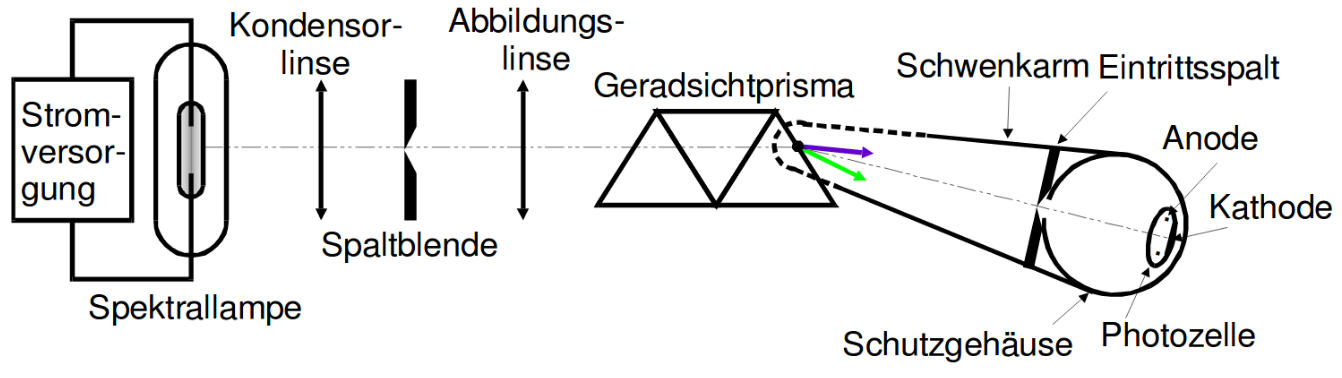
\includegraphics[width=\textwidth]{Pics/Linsensystemskizze.png}
  \caption{Schematische Darstellung des verwendeten Linsensystems}
  \label{fig:Linsensystem}
\end{figure}

Desweiteren werden für die Messung noch Apparaturen zur Bestimmung des Photostroms
und der Gegenspannung benötigt. In Abb. \ref{fig:Schaltskizze} ist ein Schaltplan
der verwendeten Messapparaturen dargestellt.

\begin{figure}
  \centering
  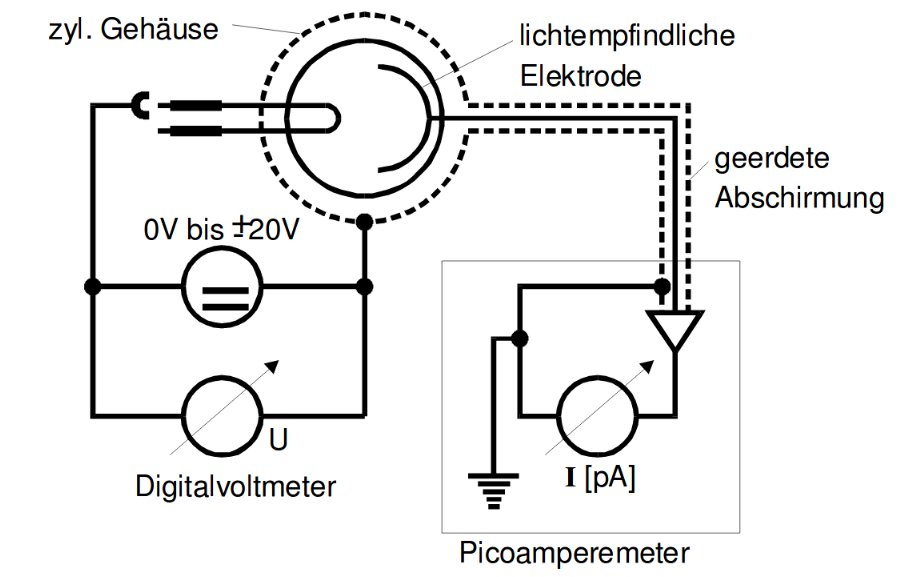
\includegraphics[width=\textwidth, height=9cm]{Pics/Schaltskizze.png}
  \caption{Schaltplan der verwendeten Messapparaturen}
  \label{fig:Schaltskizze}
\end{figure}
\FloatBarrier

Das Piccoampermeter misst den Photostrom und das Digitalvoltmeter liefert die
variable Spannung.

Zu Beginn der Messung wird das Linsensystem so justiert, dass die Spektrallinien
der $\ce{Hg}-$Quelle deutlich zu erkennen sind. Dabei ist entscheidend, dass sich
die Spektrallinien nicht überscheinden, sodass sie einzeln vermessen werden können.
Nach Beendigung der Justage wird die gelbe Spektrallinie für verschiedene Spannungen
vermessen. Die Photozelle muss so ausgerichtet werden, dass nur die gelbe Spektrallinie
in sie einfällt. Die Spannung wird auf $\SI{20}{\volt}$ geregelt, damit die
Elektronen beschleunigt werden. Die Spannung wird bei nehmen der Messwerte soweit
herunter geregelt, bis der Photostrom verschwindet. Als Messwerte werden immer
die eingestellte Spannung und der zugehörige Photostrom genommen.

Danach werden die anderen Spektrallinien vermessen. Deren Messung beginnt bei einer
Spannung von $\SI{0}{\volt}$ und wird herabgereglet, bis der Photostrom verschwindet.
Die Anzahl der Messwerte wird nach eigenem Ermessen bestimmt.
